\begin{abstract} In this work, we extended Lavrenko's relevance model and
adapted it to the cases where an additional layer of document representation is
beneficial to the application.  With this adaption, we are able to aggregate
heterogeneous data sources and operate the model in different granularity
level.  We demonstrated this idea with two real-world applications.  In the first task, we
showed the feasibility of using a carefully-selected vocabulary as the query
expansion source in a language model to enhance retrieval effectiveness.  The
proposed query refinement model outperformed the relevance model counterpart in
terms of MAP by 17.6\% under rigid relevance judgment.  Also in the second
task, we established a ranking scheme that could be used in a faceted search
session to sort the facets based on their corresponding relevance to the query.
The result showed that our approach improved the performance over the baseline
method by roughly 100\% in terms of MAP.  \end{abstract}

\section{Introduction}

Over the past few years, the abundant information on the Web along with the
rise of Web users has silently changed the usual shape of information retrieval
in the way we model documents.  A document used to be only a collection of
terms, and retrieval models were acting merely based on this piece of
information to direct user to the documents that were most likely what they
needed.  There was also a time when user-contributed tags or human annotations
were not so popular or even made available to the researchers.  Today, the
table has turned.  We have seen many successful IR applications that made use
of these external resources to improve retrieval efficiency, cases where the
use of metadata items and keywords, data that surrounds the documents that used
to be left outside of a document model, could benefit the research field.  

The presence of these augmented contents poses new challenges to researchers in
the way the retrieval model is operated on top of heterogeneous data sources.
One intuitive way to get over this problem is to mix various sources into one
distribution, which is a commonly-used technique in the literature.  Doing so,
however, might give rise to other issues since the new representation did not necessarily
share the same context with the original one, making it difficult to assign
term weights or distribute probability masses.  Recall that we have experienced
the same issue when trying to mix the contents in the document title with that
in the document body to create an single index; any attempt for adjusting the
weight of title words might end up harming theoretical soundness.

This issue has brought our attention to the possibility of building additional
layers of document representations into existing retrieval frameworks, in which
we are able to aggregate information from various sources and to operate the
model in different granularity as necessary.  Consider applications that could
take advantage of this idea, such as facilitating cross-language information
retrieval in a corpus where documents possess multiple representations over
different languages; receiving user queries in a general vocabulary while
operating the retrieval process in another level where documents are indexed
with more specific terms; or searching for named entities that are relevant to the
user queries in a collection where manually-labeled, high-quality annotations
were already made available at the document level.  

The aforementioned thoughts have motivated our research on formal retrieval
methods.  In addition to the regular term set $T$, we look {for} ways to build
a {\it secondary document representation} $S$ into a model so as to enable
simple interaction between the two layers, such as retrieving elements from one
side with that of the other as the query.  In mathematical terms, we want to
estimate the probability $\Pr(s|t)$, given that a document $d_i$ is indexed in
two different representations $T_i$ and $S_i$, where $T_i \subset T$ and $S_i
\subset S$.  A concrete application of this is to let the user form a query
$\mathbf{q} \subset T$ and estimate the probability $\Pr(s|\mathbf{q})$
accordingly.

To achieve our goal, in this paper we proposed a generalization over Lavrenko
and Croft's work \cite{lavrenko2001relevance} on relevance modeling.  The
relevance model was adapted to the cases where two individual term
distributions were available in the text collection.  We took a Bayesian
generative approach, starting from a graphical model in which documents, terms,
and hyperparameters were all explicitly specified and then broke down the
full-blown probabilistic network to a few equations that could easily
implemented at the index level.  

The rest of the work is structured as follows.  First, we introduce a Bayesian
generative process that involves two individual term distributions in
Section~\ref{s:model} and show that the process leads to a generalized relevance
model.  Then, in Section~\ref{s:experimental-results}, we present two
applications of our model.  In Section~\ref{s:query-modeling}, the idea of
query expansion in language modeling is revisited by considering user queries
in a set of terms indexed in general vocabulary and further expanding the set
by collecting relevant concepts in a more specific vocabulary; the other task
we introduce in Section~\ref{s:facet-ranking} is about named-entity ranking, in
which we use $\Pr(s|\mathbf{q})$ to sort the named entities retrieved in a facet search
session and present the entities according to their relevance to the query.  In
each task, the corresponding evaluation benchmark are also described.  We
briefly summarize the related work in Section~\ref{s:related-work}.  Finally,
we discuss a few issues arise in the development of the work and give out
concluding remarks in Section~\ref{s:concluding-remarks}.

%--------------------------------------------------
% In the past few years, faceted search has gained wide acceptance in the digital
% library and the Web community.  We have seen many successful applications of
% this technique in different domains, including the Web
% \cite{hearst2002finding}, image collections \cite{yee2003faceted}, and database
% catalogs \cite{roy2008minimum}; the technique has also given rise to a number
% of interesting research results that application developers could immediately
% benefit from, such as the usability of the faceted interface
% \cite{kules2009what} and the approach for automatically extracting facets from
% the texts \cite{mimno2007organizing}.  
% 
% We argue that a reasonable facet ranking algorithm should always assign higher
% weights to the facets discovered from the top-ranked documents; therefore, the
% algorithm itself may need to co-operate with the retrieval model for obtaining
% better facet ranking.  In this paper, we proposed one such algorithm to address
% this issue.  Our idea is to induce two document-specific distributions for each
% document: One accounts for the generation of terms, and the other the
% generation of facets.  We incorporated both distributions in a Bayesian
% framework and used the model to infer probability estimates for ranking facets.
% We conducted a series of experiments on a custom benchmark.  The result showed
% that our methods outperformed the regular count-based baseline in the facet
% ranking task, achieving promising improvement in mean-average precision and
% precision-at-10. 
%-------------------------------------------------- 

\section{Model}\label{s:model}

%--------------------------------------------------
% An intuitive way to induce a ranking scheme for facets is to consider the
% relevance scores contributed by the documents that cover the target facet.
% This can be stated as the following two criteria: \begin{itemize} \item A facet
% should receive greater weight if it is covered by a highly-relevant document and
% less weight if it is covered by an irrelevant one. \item There
% should be a way to accumulate the weights received from multiple documents.
% \end{itemize} Based on this idea, we exploit the document retrieval scores to
% model the contribution of relevance.  We find it more appealing to apply this
% technique on a language-model-based backend, since the document relevance score
% can be easily integrated into the final ranking results; the detail is
% elaborated in the upcoming sections.
%-------------------------------------------------- 

In this model, we hypothesize the existence of the two independent multinomial
distributions associated with each document $d_j$; we further assume that, in
each document, the terms observed in the \emph{primary} representation $T_j$
are drawn from the first multinomial, and those in the \emph{secondary}
representation $S_j$ drawn from the second.  The advantage of making this
independent assumption can be stated in two respects.  First, separation of the
generation processes on both sides may lead to a cleaner framework, which makes
model inference a bit easier; second, we want to highlight the fact that these
two terms sets do not necessarily share the same context and further simplify
the dependency relations in the resulting Bayesian network.  

\subsection{The Generative Framework}

Figure~\ref{f:model} shows our proposed Bayesian generative framework.
Consider the collection is composed of $N$ documents, in which each document
$d_j$ is associated with two sets of terms $T_j$ and $S_j$.  We refer $T_j$ as
the primary representation and $S_j$ the secondary representation.  Each
document $d_j$ possesses two multinomial distributions, denoted by $\tau^{(j)}$
and $\phi^{(j)}$, from which elements in $T_j$ and $S_j$ are drawn
independently.  The two multinomials for a document could also be understood as
two independent document models $p(w|\tau^{(j)})$ and $p(w|\phi^{(j)})$ that
work on two different sets of vocabularies.  Two Dirichlet distributions
$\{\alpha_i; i \in [1, |T|]\}$ and $\{\beta_k; k \in [1, |S|]\}$ are assumed in
the model to govern the generation of these multinomials.  

\begin{figure}[ht!]
  \centering
  \psset{xunit=10mm,yunit=8mm}
  \begin{pspicture}(0,-2)(8,5)%\showgrid  % Uncomment to show grid!
    \SpecialCoor  % (a|b) means x-coord from 'a' and y-coord from 'b'.
    \psset{arrowscale=1.5}
    \rput(4.0,0.0){\GM@node[observed=true]{d}}\GM@label[angle=90]{d}{$d_j = j$}
    \rput(2.0,0.0){\GM@node[observed=true]{t}}\GM@label[angle=45]{t}{$t_i$}
    \rput(1.25, -0.75){\GM@plate{1.5}{1.5}{$|T_j|$}}
    \rput(6.0,0.0){\GM@node[observed=true]{s}}\GM@label[angle=45]{s}{$s_k$}
    \rput(5.25, -0.75){\GM@plate{1.5}{1.5}{$|S_j|$}}
    \rput(0.75, -1.25){\GM@plate{6.5}{2.5}{$N$}}

    \rput(4.0,4.0){\GM@node{x}}\GM@label[angle=45]{x}{$x$}
    \rput(2.0,4.0){\GM@node[observed=true]{q}}\GM@label[angle=45]{q}{$q_i$}
    \rput(1.25, 3.25){\GM@plate{1.5}{1.5}{$|Q|$}}
    \rput(6.0,4.0){\GM@node{y}}\GM@label[angle=45]{y}{$y$}

    \rput(2.0,2.0){\GM@node{tau}}\GM@label[angle=45]{tau}{$\tau$}
    \rput(6.0,2.0){\GM@node{phi}}\GM@label[angle=45]{phi}{$\phi$}
    \rput(0.0,0|tau){\GM@parameter{alpha}}\GM@label[angle=45]{alpha}{$\alpha$}
    \rput(8.0,0|phi){\GM@parameter{beta}}\GM@label[angle=45]{beta}{$\beta$}

    \ncline[arrows=->]{d}{t}
    \ncline[arrows=->]{d}{s}
    \ncline[arrows=->]{x}{q}
    \ncline[arrows=->]{x}{y}
    \ncline[arrows=->]{tau}{t}
    \ncline[arrows=->]{tau}{q}
    \ncline[arrows=->]{phi}{s}
    \ncline[arrows=->]{phi}{y}
    \ncline[arrows=->]{alpha}{tau}
    \ncline[arrows=->]{beta}{phi}
  \end{pspicture}

  \caption{The document-centric generative model is shown in the plate
  notation, in which shaded nodes denote observed variables.  The document
  $d_j$ generates two representations $T_j$ and $S_j$, where each term in $T_j$
  is represented as $t_i$ and that in $S_j$ represented as $s_j$.  The query
  terms are represented as $q_i$'s, which are drawn from an unknown document
  model $x$; the document is associated with an unknown term $y \in S$.} \label{f:model}
\end{figure}

As suggested in the upper-half of Figure~\ref{f:model}, the input query
$\mathbf{q}$ is modeled as a set of observed terms drawn from an unknown
document model $x$ in the collection.  Specifically, the query terms are
encoded in the same vocabulary as in that form the primary representation of
document $x$.  By making this assumption, we are able to match the query
against all the document models and to estimate the query likelihood
$\Pr(\mathbf{q}|d_j)$.  This leads us to the probabilistic generative methods,
such as language modeling.  Recall that the unknown document $x$ is connected
to another unknown variable $y$.  The variable $y$ represents the most probable
term generated from the secondary multinomial distribution $\phi^{(x)}$.

The entire generative process can be summarized as follows:
\begin{enumerate} 
  \item For each document $d_j$, \begin{enumerate}
    \item $\tau^{(j)} \sim \textrm{Dirichlet}(\alpha_i; i \in [1, |T|])$
    \item $\phi^{(j)} \sim \textrm{Dirichlet}(\beta_k; i \in [1, |S|])$
    \item For $i \in \{ 1, \ldots, |T_j| \}$, $t_i \sim \textrm{Mult}(\tau^{(j)})$ 
    \item For $k \in \{ 1, \ldots, |S_j| \}$, $s_k \sim \textrm{Mult}(\phi^{(j)})$ 
  \end{enumerate}
  \item For some unknown document $d_x$, \begin{enumerate}
    \item For $i \in \{ 1, \ldots, |\mathbf{q}|\}$, $q_i \sim \textrm{Mult}(\tau^{(x)})$
  \end{enumerate}
\end{enumerate}

\subsection{Inference}

The discussions have brought us to the focus of this work, which is to explicitly
estimate the likelihood of one term $s$ in the secondary term domain being
triggered\footnote{We coin the term due to lack of obvious dependency
between both sides.} by another set of terms from the primary term
domain.  This task can be framed as a optimization problem:
\begin{equation} y^* = \arg\max_{y \in S} \Pr(y|\mathbf{q}, \mathbf{t},
\mathbf{d}, \mathbf{s}) \label{eq:forward} \end{equation} where $\mathbf{t}$
and $\mathbf{s}$ represent all the observed terms in the primary/secondary
representations in the collection, respectively; $\mathbf{q}$ represents
the input query and $\mathbf{d}$ denotes all the observed documents.  The 
right-hand-side of Equation~\eqref{eq:forward} can be broken down into the following form:
\begin{eqnarray}
  \Pr(y|\mathbf{q}, \mathbf{t}, \mathbf{d}, \mathbf{s}) 
  &=& \sum_{x \in [1, N]} \Pr(y|x, \mathbf{q}, \mathbf{t}, \mathbf{d}, \mathbf{s}) \Pr(x|\mathbf{q}, \mathbf{t}, \mathbf{d}, \mathbf{s}) \nonumber\\
  &\propto& \sum_{x \in [1, N]} \left\{ \int \Pr(y|x, \phi^{(x)}) \Pr(\phi^{(x)}|d_x, \mathbf{s_x}) \mathrm{d}\phi^{(x)} \right. \nonumber\\
  && \left. \int \Pr(\mathbf{q}| x, \tau^{(x)}) \Pr(\tau^{(x)}|d_x, \mathbf{t_x})\mathrm{d}\tau^{(x)} \Pr(x) \right\} \nonumber\\
  &=& \sum_{x \in [1, N]} \frac{\beta_y + c_{y,x}}{\sum_k \beta_k + c_{k,x}} \frac{\mathcal{B}(\{\alpha_i + c_{i,x} + c_{i,q} \})}{\mathcal{B}(\{\alpha_i + c_{i,x} \})} \Pr(x) \label{eq:forward-solution}
\end{eqnarray}
The last line follows the conjugacy of Dirichlet distribution, as in:
\begin{eqnarray*}
\Pr(\phi^{(x)}|d_x,\mathbf{f_x}) &\sim& \mathrm{Dirichlet}(\{\beta_k + c_{k,x}; \forall k \}) \\
\Pr(\tau^{(x)}|d_x, \mathbf{t_x}) &\sim& \mathrm{Dirichlet}(\{\alpha_i + c_{i,x}; \forall i \}).
\end{eqnarray*}
Recall that $\mathcal{B}(\cdot)$ is the multinomial beta
function defined by \[\mathcal{B}(a_1, \ldots, a_n) = \frac{\prod_i
\Gamma(a_i)}{\Gamma(\sum_i a_i)}. \]

\subsection{Hyperparameters and Index Structure}

Another issue that we would like to address in this work is the choice of
priors.  Consider a prior as a vector of size $|S|$: $(\beta_1, \beta_2,
\ldots, \beta_{|S|})$.  There are two particular prior distributions that we
want to study in this work.  The first one is the \emph{uniform} prior: \[ (c, c,
\ldots, c), \] in which we let $\beta_k = c$ for each $k \in [1, |S|]$ and $c$
denote some constant.  The second one is called \emph{smoothed-Dirichlet},
which is widely-used as a smoothing method in the language modeling
applications for information retrieval \cite{zhai2004study}: \[ (\mu
\Pr(s_1|C), \mu \Pr(s_2|C), \ldots, \mu \Pr(s_{|S|}|C)), \] where $\Pr(s_k|C)$
denotes the probability of generating term $s_k$ (in the secondary
term domain) from the collection by viewing the entire collection as one
language model; $\mu$ represents some constant.

One interesting feature of our model is that it offers seamless integration
with the language-model-based retrieval method.  It comes from
the fact we could further simplify Equations~\eqref{eq:forward-solution} by
assigning $\alpha$ as a smoothed-Dirichlet prior and $\Pr(x)$ as a uniform
prior.  When $\alpha_i = \mu \Pr(t_i|C)$, it can be shown that: \[
\frac{\mathcal{B}(\{\alpha_i + c_{i,x} + c_{i,q} \})}{\mathcal{B}(\{\alpha_i +
c_{i,x} \})} \propto {\rm L}_{\rm LM}(\mathbf{q}|d), \] where ${\rm L}_{\rm
LM}(\mathbf{q}|d)$ denotes the query likelihood score in the language model
with Dirichlet smoothing scheme.  In this case, the model scores becomes:
\begin{eqnarray*}
  \Pr(y|\mathbf{q}, \mathbf{t}, \mathbf{d}, \mathbf{s}) &\propto& 
  \sum_{x \in [1, N]} \frac{\beta_y + c_{y,x}}{\sum_k \beta_k + c_{k,x}}
  {\rm L}_{\rm LM}(\mathbf{q}|x) \nonumber\\
\end{eqnarray*} 

\section{Experimental Results}\label{s:experimental-results}

In this section, we introduce two applications of our proposed framework.  In
the first experiment, we use a different set of terms to refine the query model
so as to leverage retrieval effectiveness; in the second experiment, we showed
that we were able to retrieve the named entities relevant to the user query
from a database by supplying the entities as the secondary document
representation.  Both experiments were conducted in a way that is general
enough so that the result could be reproduced by any follow-up research.

\subsection{Query Refinement Using the Secondary
Representation}\label{s:query-modeling}

The probability estimate $\Pr(y|\mathbf{q}, \mathbf{t}, \mathbf{d},
\mathbf{s})$ that we obtained from the proposed model can be seen as a
\emph{refined query model}, an idea that has been proposed in
\cite{lavrenko2001relevance}.  In this case, we can employ a two-stage
retrieval strategy to enhance retrieval performance.  First, We made an initial
retrieval run to populate a refined model, and then re-submit the model as a
new query to the retrieval system.  What makes our approach different from the
original relevance model, however, is the presence of the secondary document
representation; in Lavrenko's work, only one document
representation was assumed.

The major obstacle for realizing such type of model-based query refinement lies
in the restriction of the language modeling framework, according to which the
input query should always be specified as a sequence of terms, each associated
with an positive integer indicating the corresponding number of occurrences in
the query text.  We developed a technique that enabled a second-round retrieval
in our study by \emph{realizing} the probability distribution
$\Pr(y|\mathbf{q}, \mathbf{t}, \mathbf{d}, \mathbf{s})$ as a sequence of
\emph{expected terms}.  This can be done through the construction of a
very-long, pseudo-query sequence.  We begin by incorporating all the term $s_k$
in the secondary representation, and then take the conditional expectation
$\mathrm{E}(s_k|\mathbf{q}, \mathbf{t}, \mathbf{d}, \mathbf{s})$ for each term
$s_k$ as the corresponding number of occurrences in the new query.  It can be
shown that this simple technique reduces to the KL-divergence retrieval
framework proposed in \cite{zhai2001language}. 

The benchmark corpora that we used to testify the proposed solution was the
NTCIR-4 Test Collection.  The particular task that we considered here is a
subtask of the NTCIR-4 CLIR Task: Chinese-to-Chinese monolingual document
retrieval.  The dataset comprised of totally 381,681 newswire articles and 59
test topics.  We used only title queries in this experiment.

We took limited preprocessing steps to the corpus.  First, we scanned
through each document and identified a number of text segments; all the
unrecognized texts, such as punctuation marks or symbols, were discarded
immediately.  A text segment of interest could be formed by either (i) one or more consecutive CJK
characters, or by (ii) one or more English words separated by hyphens or
whitespaces.  Then, we further broke down these text segments into a number of tokens
using the following processing rules:  \begin{itemize} \item For each text
segment of category (i), output the bigrams obtained from the character
sequence, i.e., the expected output for a given text segment $w_1 w_2 w_3
\ldots w_n$ is $\{ w_i w_{i+1} | i \in [1, n-1] \}$.  \item For each text
segment of category (ii), output the words by splitting the text with whitespaces or
hyphens.  \end{itemize} 

The resulting token stream was a mixture of CJK-character bigrams and English
word unigrams, which formed the primary document representations in our model
and in other baseline methods.  Meanwhile, the secondary representation we
chose was the top-500000 CJK-character bigrams in the entire collection ranked
by the corresponding \emph{tf-idf} score; the candidate set was formed by
excluding those bigrams whose occurrence is less than 5.  The idea behind such
an arrangement was to retrieve the initial result from an index with general
vocabulary, to refine the query model with the highly-discriminative terms, and
obtain the final result from the secondary index.  The parameters described
here were determined through experimentation.

Our model was implemented with C++, and the rest of the experimental runs were
established on top of the Lemur toolkit.  From all the retrieval methods
supported by the tool, we selected tf-idf, okapi, and indri (a
language-model-based method) as the baseline methods.  Standard query expansion
techniques for each selected method were also supported in the Lemur toolkit.
Pseudo-relevance feedback was implemented for both tf-idf and okapi models, and
an adaptation of Lavrenko's relevance model was also built into the core of
Indri index.  In the regular runs, we stuck with the default parameter values
{for} all the participant models; when employing pseudo-relevance feedback, we
set the number of feedback documents as 20 and the number of feedback terms as
100.  In our own refinement model, the refined query was computed under the
same restriction, where terms other than the top-ranked 100's were completely
ignored.  Recall that our model reviewed all the retrieved top-1000 documents
to achieve the probability estimates.  The performance is measured in terms of
mean average precision and precision-at-5.  

\begin{table}[ht!]
  \centering
  \begin{tabular}{llllll}
    Method & & MAP (+\%) & P@5 (+\%) & MAP (+\%) & P@5 (+\%) \\
    \hline
    {\tt tfidf} & & 0.181 & 0.264 & 0.213 & 0.335 \\
    {\tt tfidf} + PRF & & 0.217 (+19.9\%) & 0.295 (+11.7\%) & 0.264 (+23.9\%) & 0.383 (+14.3\%) \\
    {\tt okapi} & & 0.185 & 0.278 & 0.223 & 0.356 \\
    {\tt okapi} + PRF & & 0.224$^{**}$ (+21.1\%) & 0.315 (+13.3\%) & 0.270$^{**}$ (+21.1\%) & 0.400 (+12.4\%) \\
    \hline
    {\tt indri} & & 0.174 & 0.258 & 0.216 & 0.346 \\
    {\tt indri} + Relevance & & 0.180 (+3.4\%) & 0.271 (+5.3\%) & 0.222 (+2.8\%) & 0.342 (-1.2\%) \\
    {\tt lm} & & 0.170 & 0.251 & 0.209 & 0.322 \\
    {\tt lm} + Refinement & & 0.207$^*$ (+21.8\%) & 0.302 (+20.3\%) & 0.261$^*$ (+24.9\%) & 0.369 (+14.6\%) \\
    \\
  \end{tabular}

  \caption{The result for the query refinement task.  Retrieval methods listed in the
  upper-half are tfidf-based, while those in the lower-half are
  language-model-based.  The overall top-performer is indicated with two
  asterisks in the superscript, while the best run in the language-modeling
  side is indicated with one asterisk.}
  \label{t:query-modeling}
\end{table}

Table~\ref{t:query-modeling} shows the experimental result.  The overall best
performance fell on the okapi + PRF run, achieving 0.224 under rigid judgment
and 0.270 under relax judgment in terms of MAP.  Even though our proposed
method achieved roughly comparable performance as tfidf + PRF, the difference
between the performance of tfidf-based methods and that of language-model-based
methods remains rather significant.  Generally, the performance for all the
expansion runs can be summarized as okapi + PRF $>$ tfidf + PRF $>$ lm + refinement
$>>$ indri + relevance.

Among all the regular runs, our language modeling implementation achieved the
lowest MAP under both judgment sets; the retrieval performance was greatly
improved when refinement model was applied, achieving 0.207 for rigid relevance
judgment and 0.261 for relax in terms of MAP.  The proposed query refinement
model outperformed the relevance model built into the Indri index.  Since our
proposed model can be viewed as a relaxed (or adapted) version of the original
relevance model, this encouraging result partly confirmed our hypothesis that
bad expansion terms could be avoided by biasing the expansion source toward a
secondary document representation that possesses a cleaner,
highly-discriminative vocabulary.  

\subsection{Retrieving Query-Relevant Facets}\label{s:facet-ranking}

Faceted search \cite{hearst2002finding,yee2003faceted,roy2008minimum} can be
seen as a two-phase extension of the ordinary retrieval task: In the first
phase, one populates a set of documents (the \emph{result set}) by querying the
underlying retrieval model; then, in the second phase, one exploits the
associations between the facet entries and the documents, and returns the facet
items back to the users.  The collected facets are usually presented in
descending order of the corresponding number of occurrences in the result set,
which we called the \emph{count-based scheme}.  The scheme is mostly preferable
because it is fast and easy to implement.  However, it treats all the collected
facet counts equally important and disregards the differences on the degree of
relevance between the retrieved documents.  In other words, a facet found in a
low-rank document might appear as good as that found in a top-rank one when
this simple ranking scheme is employed.

This can also be a problem when the user wants to consult the retrieved facets
to guide the subsequent exploratory search.  Since the facets are not sorted in
terms of relevance, the user might be mislead by top-ranked facets that are not
actually relevant to input query but merely make it to the top by being
commonly referred in low-ranked documents.  We argue that a reasonable facet
ranking algorithm should always assign higher weights to the facets discovered
from the top-ranked documents; therefore, the algorithm itself may need to
co-operate with the retrieval model for obtaining better facet ranking.  This
observation has brought us to a simple solution: We can build in the facets
associated with each document as a secondary representation and utilize
Equation~\ref{eq:forward-solution} to rank the facets.  

%--------------------------------------------------
% The test corpus that we chose is the Tan-Hsin Archive \zhtw{(淡新檔案)}, which
% is currently the most sizable and complete collection of historical documents
% in Taiwan dating back from 1776 to 1895.  
%-------------------------------------------------- 

The very nature of this task makes our proposed model feasible.  One major
difficulty that we faced, however, was the lack of standard benchmark on the
facet ranking task.  As a result, we went for a custom benchmark based on one
text collection in our own applications.  The test corpus that we chose was
XXXXXXXX\footnote{Removed due to double-blind review}, which is currently the
most sizable and complete collection of historical documents in XXXXXXXX.  We
took a subset of 15,314 documents from the collection to form the test set.
Each document in the collection was associated with a set of human-annotated
facets.  By considering topic coverage and ease of evaluation, we tested model
performance only on person names as the designated facet set.

%--------------------------------------------------
% The number of unique person names in the dataset is 10,918, and the total
% number of occurrences of these facets is 37,489.  Thus, the average number of
% person names associated with a document is 2.45.  All these information were
% already made available in the metadata of the documents.  
%-------------------------------------------------- 

To prepare the query topics, we first fetched all the query log entries from
the database server.  We put together a set of 105 query topics, each of which
had obtained more than 50 hits in our database.  We randomly chose 28 topics
out from the set and used them in the following evaluation.  The relevance
judgment was made manually.  For each query topics, we prepared a list of
the top 100 facets returned by the baseline retriever that operated merely
based on occurrence counts; the domain expert would then go over the entire
list, labeling each facet as relevant or irrelevant accordingly.
We considered 3 competing runs in the experiment: (i) {\tt baseline}, with
which facets were ranked by the corresponding number of counts in the result
set; (ii) {\tt uniform-prior}, with which facets were ranked by the proposed
model using uniform prior for $\beta$; and (iii) {\tt smoothed-prior}, with
which facets were ranked by the proposed model using Dirichlet-smoothed prior
for $\beta$. 

We took the top-1000 documents retrieved by using Dirichlet-smoothed language
model with $\mu = 2,500$ as the result set.  The hyperparameter was
pre-determined through experimentation.  All the algorithms took the same set
of document IDs as input.  For our proposed methods, we reused the retrieved
scores returned by the document-level retrieval model, as stated in the
preceding sections.  The output was a sorted list of all the associated facets
in descending order of the ranking score.  For efficiency, we used only the
top-100 facets returned by each run as the final results.  The performance was
assessed both in terms of mean-average precision (MAP) and precision-at-10
(P@10).  

\begin{table}[ht!]
  \centering
  \begin{tabular}{llll}
    Method & & MAP & P@10 \\
    \hline
    {\tt baseline} & & 0.2996 & 0.3857 \\
    {\tt uniform-prior} & $\beta = 0$ & 0.5775 & 0.6179\\
    & $\beta = 1$ & 0.5899$^*$ & 0.6464$^*$ \\
    & $\beta = 10$ & 0.5877 & 0.6464$^*$ \\
    {\tt smoothed-prior} & $\mu = 0.01$ & 0.5781 & 0.6179 \\
    & $\mu = 1$ & 0.5782 & 0.6214 \\
    & $\mu = 100$ & 0.4956 & 0.5429 \\
    \\
  \end{tabular}
  \caption{The performance results for all the test runs.  The top-performer is indicated by an asterisk in the superscript.}
  \label{t:performance}
\end{table}

The performance of the baseline method was quite moderate, with MAP a bit less
than 0.3 and P@10 around 0.39.  That means, in general, users might find 4 out
of the top-10 facets relevant to the query topic.  The reported P@10 value met
our expectation; however, a higher MAP value was expected for the baseline
between 0.33 and 0.35.  All the proposed models show significant improvement
over the baseline, ranging from 30\% to 100\% in terms of MAP.  Encouraged by
the initial results, we ran a line search for each model by varying the
hyperparameter $\beta$.  We found that model performance were quite stable
across different experimental runs.  Generally, {\tt uniform-prior} and {\tt
smoothed-prior} achieved comparable performance.  The best one was found in the
{\tt uniform-prior} run with $\beta = 0.2$, achieving $0.591$ in MAP.  The
positive observation in this experiment suggested that a relevance-based
weighted-sum model is probably more effective than a count-based model in the
facet ranking task.  

Recall that the result also suggested that the simple uniform prior could be 
superior to the smoothed prior, though only to a limited degree.  This may
indicate that, at least in our test collection, the prior $\Pr(y|C)$ did not
make good estimation for $\Pr(y|d)$.  We also found that models with
zero prior (i.e., $\beta = 0$) were in fact among the top-performer of the
ranking task, suggesting that using the maximum likelihood estimate alone might
fit the data well enough.  A further investigation into the data is needed to
explain why incorporation of the smoothed prior might wash away the influence
of the maximum likelihood estimates.

%--------------------------------------------------
% \begin{figure}[ht!]
%   \centering
%   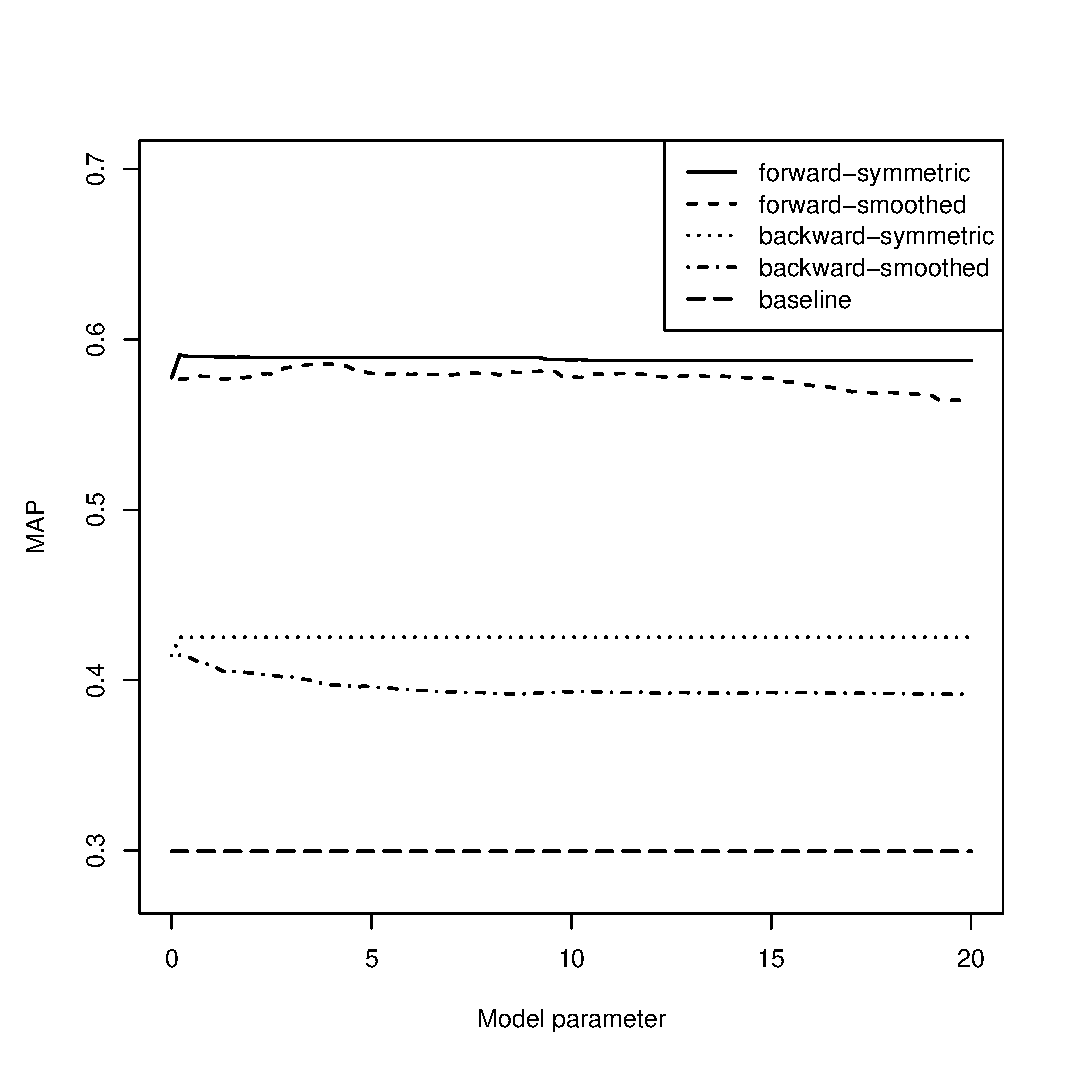
\includegraphics[width=10cm]{performance.eps}
%   \caption{The performance results for all the test runs.  The x-axis indicates
%   the model parameter: $\beta$ in symmetric model and $\mu$ in smoothed model.
%   The y-axis indicates the resulting MAP values.  This figure shows the
%   proposed ranking models outperforms the baseline approach across different
%   settings of parameters.} \label{f:performance}
% \end{figure}
%-------------------------------------------------- 

\section{Related Work}\label{s:related-work}

Our proposed framework was inspired by the recent advances on language modeling
applications in information retrieval
\cite{lavrenko2001relevance,zhai2001language,zaragorza2003bayesian}.  In this
respect, our solution can be seen as a two-stage extension of the regular
language model over the facet data.  Our approach differs from the conventional
language modeling methods in the presence of a secondary document
representation.  

To the best of our knowledge, this work is among the earliest attempt for
retrieving relevant facets in the digital library community.  Interestingly, we
learned that similar attempts were made in the area of expert finding.  In
\cite{amitay2008finding}, Amitay et al. formulated the problem of expert
finding as a two-layered retrieval task and proposed a solution based on the
\emph{inverse entity-frequency} that achieved moderate performance on the task.
Balog et al. \cite{balog2009language} followed up in the same direction by
proposing a language modeling framework with the similar rationale to extend
the use of language model to the underlying co-occurrence statistics by
exploiting person-term and person-document links.  Our contribution departs
from these two previous efforts, not only in the application domain, but in the
way document relevance is incorporated into the model and the support for prior
belief.  
 
\section{Discussion and Concluding Remarks}\label{s:concluding-remarks}

In this work, we proposed a Bayesian framework that enabled the use of a
secondary document representation in language modeling.  The framework extended
Lavrenko's relevance model to offer interoperability between two different
term domains.  Moreover, we showed that our method is capable of working with a
language-model-based retrieval engine to achieve high efficiency in
computation.  

Two applications were introduced in this paper to evaluate the performance of
the proposed solution.  In the first task, we showed that the presence of a
secondary document layer that is made of a carefully-selected vocabulary could
greatly enhance retrieval effectiveness.  Even though the proposed query
refinement model did not achieve the best performance, the model still beaten
the relevance model baseline by 17.6\% (rigid) and 22.7\% (relax) in term of
MAP and gained comparable performance as {\tt tfidf} with pseudo-relevance
feedback.  The refinement model alone improved the MAP of the regular language
modeling run by 21.8\% (rigid) and 24.9\% (relax).  In the second application,
where the model was used to rank named entities returned in the query session
by the underlying retrieval system, the proposed solution achieved encouraging
result on the custom benchmark.  The baseline performance was improved by
roughly 100\% in MAP.  

Despite the early success in the evaluation results, there is still room for
improvements.  We see our contributions here as a starting point toward further
exploration on several issues that have not yet been covered in this study: the
use of different prior families, the formal inference model for the
hyperparameters, potential applications on other datasets, etc.  These
challenges should be the focus of our future work.

%--------------------------------------------------
% Another interesting aspect that we discovered in the development of testbed
% systems is that users tend to follow top-ranked facets.  According to our
% internal study on the click-through log, the average click-through rank of the
% facets falls in the top 20\% of the presented facets.  This fact also motivates
% our research toward integration of relevance into faceted interface, in which
% users could gain better insight of the content even though they do not explicit
% go through every facet that we discovered.
%-------------------------------------------------- 

\section*{Acknowledgments}

We thank XXXXXXXX\footnote{Removed due to double-blind review} for his
support on preparation of the test data.  The research efforts described in
this paper were supported under the XXXXXXXX (Project No. XXXXXXXX), which is
sponsored by XXXXXXXX.

%--------------------------------------------------
% We thank Po-Yu Chen for his support on preparation of the test data.  The
% research efforts described in this paper are supported under the National Taiwan
% University Digital Archives Project (Project No.  NSC-98-2631-H-002-005), which
% is sponsored by National Science Council, Taiwan. 
%-------------------------------------------------- 
